\section{Running MNPE}

MNPE runs from the command line. The current working directory must contain the 8 \texttt{*.inp} files. Since reading the output requires the use of Matlab scripts \texttt{peout1.m} and \texttt{peout2.m}, it is convenient to execute MNPE from Matlab also. This can be done with \texttt{system('MNPE2D')}, if the MNPE executable is on the user's system \texttt{PATH}. To execute a local copy of the executable use \texttt{system('./MNPE2D')}.

While MNPE runs, it prints updates to the command line to indicate progress to the user. It processes each frequency sequentially, printing the current frequency followed by periodic range updates. An example is shown in Listing~\ref{lst:runoutput}.

\lstinputlisting[firstline=7,caption={MNPE command line output},label={lst:runoutput}]{../images/RunOutput.txt}

Running MNPE generates binary output files \texttt{press.bin}, \texttt{apvr.bin}, and \texttt{apvz.bin}. To read and plot the outputs, run \texttt{peout1} and \texttt{peout2} from the Matlab command prompt. The scripts can either be copied into the MNPE working directory and run from there, or they can be saved in a directory that is included in the Matlab \texttt{PATH}.

The first script to run is \texttt{peout1}, which reads header data from the binary files. The script will prompt the user for the name of the file to be read. After the file name is entered by the user, the script loads that data into the Matlab workspace and displays information from the file header, as shown in Listing~\ref{lst:peout1output}. The header includes information about the run, including the actual sampling used in depth and range. These may differ from the ``requested'' values in \texttt{pefiles.inp}.

\lstinputlisting[firstline=3,caption={\texttt{peout1} output for \texttt{press.bin}},label={lst:peout1output}]{../images/peout1Output.txt}

After reading the header, the field data can be extracted by running \texttt{peout2}. It will prompt the user with multiple options, as shown in Table~\ref{tab:peout2options}.

\begin{table}[!ht]
	\begin{center}
		\caption{Options available for \texttt{peout2}}
		\label{tab:peout2options}
		\begin{tabular}{c|l} 
			\textbf{Option} & \textbf{Description}\\
			\hline
			1 & Starting field data \\
			2 & Data for single radial \\
			3 & Data for single range \\
			4 & Data for single depth \\
			5 & Data for single interface \\
			6 & Travel time data \\
		\end{tabular}
	\end{center}
\end{table}

Option 1 outputs the starting field as a function of depth and frequency in the variable \texttt{psi0}. Option 2 outputs the field as a function of depth and range in the variable \texttt{press}. The user is prompted to select a single frequency when data for multiple frequencies was calculated. The variable name \texttt{press} is used for velocity data as well as pressure data, so the user must rename this variable to prevent subsequent calls to \texttt{peout} from overwriting it. Option 3 prompts the user for a single range and outputs field data as a function of depth and frequency for that range in \texttt{press}. Similarly, Option 4 prompts the user for a single depth and outputs field data as a function of range and frequency for that depth in \texttt{pressd}. When the user selects option 5, \texttt{peout2} prompts the user to select either the water/bottom interface or bottom/deep bottom interface and then outputs the field at that interface's depth as a function of range and frequency in \texttt{pressd}. Unlike option 4, option 5 follows the bathymetry in a range-dependent environment. 

Option 6 can be used when the source input file specifies multiple frequencies.  The processing assumes a power of 2 number of frequencies
$N_f$, and defaults to a Hanning source amplitude spectrum across the bandwidth $BW$.  The user must ensure that the frequency sampling, defined by $BW/(N_f-1)$, is sufficient to avoid wrap-around of the travel time results.

Within option 6, there are multiple sub-options.  Sub-option 6.1 computes the broadband travel time data along a single radial at a specified range. Furthermore, within this sub-option, one can choose between simply producing a plot of time vs. depth, or producing a plot of time vs. vertical arrival angle, as could be processed by a vertical array through standard wavenumber processing techniques.  This latter option will also ask the user to define the upper and lower depths of the vertical array to process beams. Sub-option 6.2 computes the broadband travel time data at a single depth. The subsequent plot displays travel time vs.range. Sub-option 6.3 is similar to 6.2, but computes the broadband travel time data at an interface.

After generating plots, the user is prompted with the option to save the data to a \texttt{.mat} file. The output data remains in the current Matlab workspace even if the user does not save it to a \texttt{.mat} file. A selection of commonly-used workspace variables is listed in Table~\ref{tab:peoutdata}.

\begin{table}[!ht]
	\begin{center}
		\caption{Selected workspace variables generated by \texttt{peout1} and \texttt{peout2}}
		\label{tab:peoutdata}
		\begin{tabular}{c|l} 
			\textbf{Name} & \textbf{Description}\\
			\hline
			\texttt{nf} & Number of frequencies \\
			\texttt{nrout} & Number of points in range vector \\
			\texttt{nzout} & Number of points in depth vector \\
			\texttt{freq} & Frequency vector [Hz] (1 x \texttt{nf})\\
			\texttt{freqout} & Frequency selected by user [Hz] \\
			\texttt{rngout} & Range selected by user [km] \\
			\texttt{depout} & Depth selected by user [m] \\
			\texttt{rng} & Range vector [km] (\texttt{nrout}  x 1)\\
			\texttt{dep} & Depth vector [m] (1 x \texttt{nzout})\\
			\texttt{surf} & Ocean surface vector [m] (\texttt{nrout}  x 1)\\
			\texttt{bath} & Bathymetry vector [m] (\texttt{nrout}  x 1)\\
			\texttt{dbath} & Deep bathymetry vector [m] (\texttt{nrout}  x 1)\\
			\texttt{press} & Complex transmission loss data \\
		\end{tabular}
	\end{center}
\end{table}

\subsection{Example outputs}

The following examples are included with the MNPE distribution to demonstrate the basic features and usage of MNPE. The user is encouraged to recreate these plots with their MNPE application to verify their application is working as intended. Note that in these plots, the color scale has been changed from the default values.

\subsubsection{Flat}

The Flat environment is a 200 m deep waveguide of constant depth, with a constant sound speed of 1500 m/s. The fluid bottom has sound speed 1700 m/s, density 1.5 g/cm$^3$, and attenuation 0.333 dB/m/kHz. There is no deep bottom. The source is at a depth of 100 m, producing a single tone at 200 Hz.

\begin{figure}[!ht]
\begin{center}
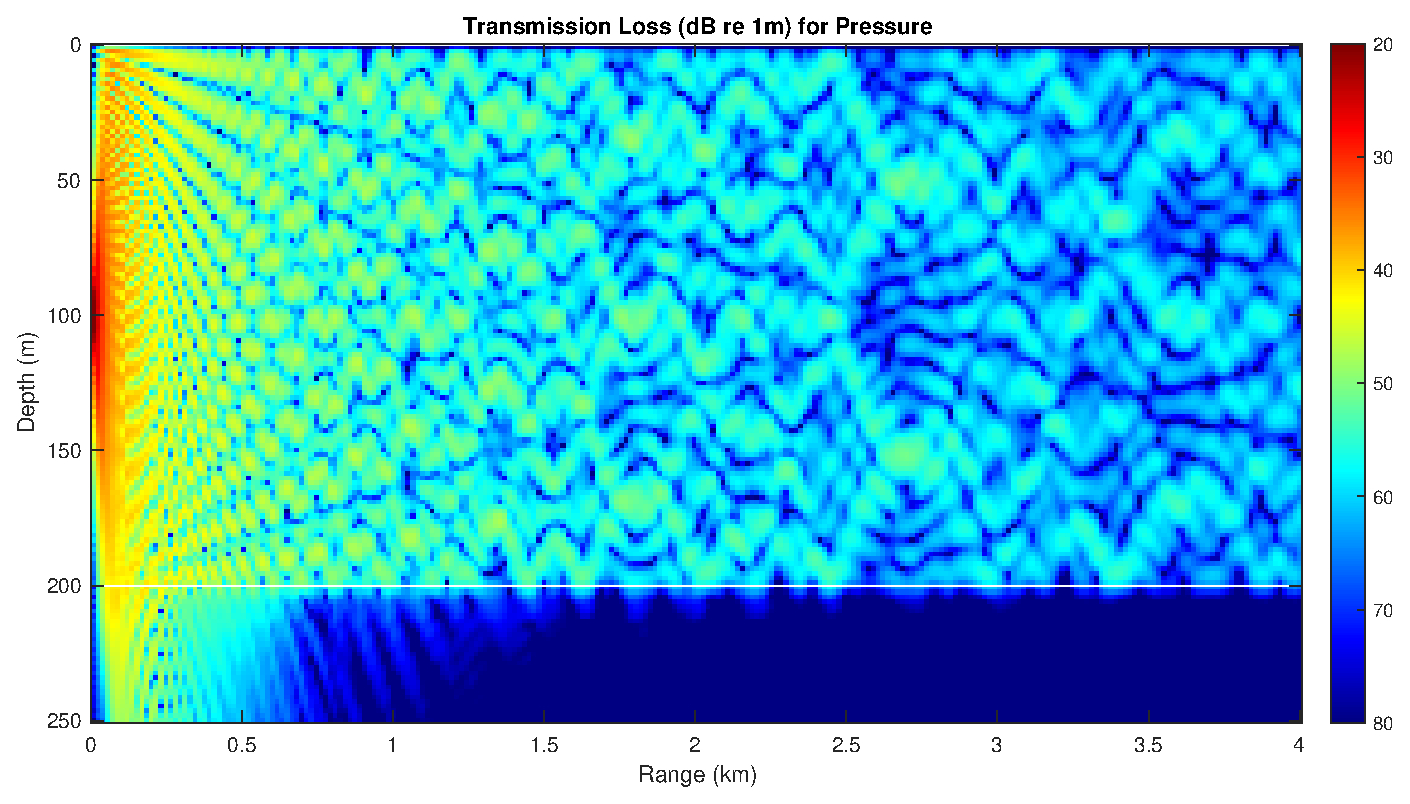
\includegraphics[width=\textwidth]{FlatP.eps}
\caption{\label{fig:FlatP}Flat environment pressure transmission loss}
\end{center}
\end{figure}

\clearpage
\subsubsection{ASA Wedge}

The ASA Wedge environment is identical to the Flat environment, except that the bathymetry varies linearly from 200 m at range 0 km to 0 m at range 4 km. The source is again at a depth of 100 m, producing a single tone at 200 Hz.

\begin{figure}[!ht]
\begin{center}
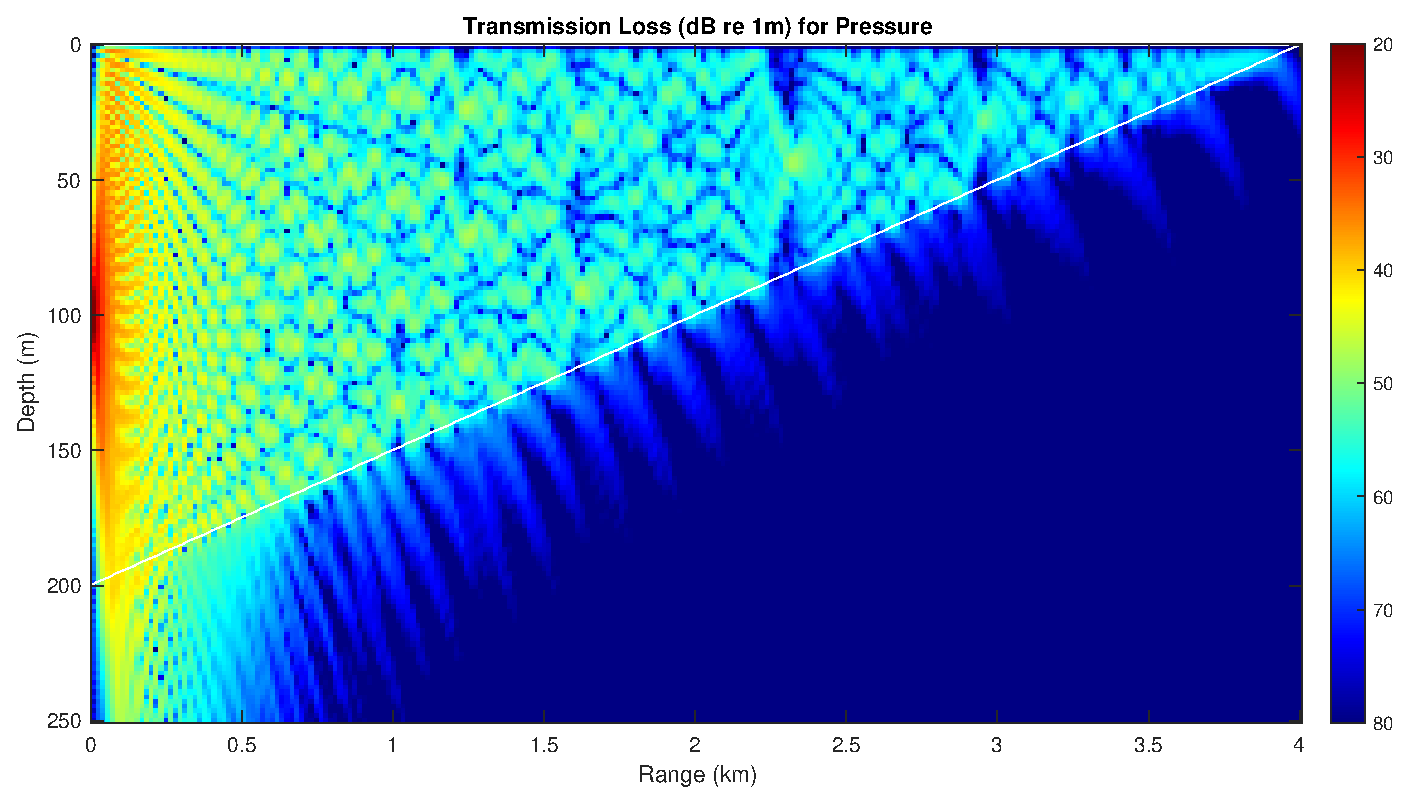
\includegraphics[width=\textwidth]{ASAWedgeP.eps}
\caption{\label{fig:ASAWedgeP}ASA Wedge environment pressure transmission loss}
\end{center}
\end{figure}

\clearpage
\subsubsection{Monopole Source}

This example demonstrates pressure and vertical velocity outputs for a monopole source in the Flat environment with 100 m bathymetry. The source is at a depth of 50 m, producing a single tone at 60 Hz.
 
\begin{figure}[!ht]
\begin{center}
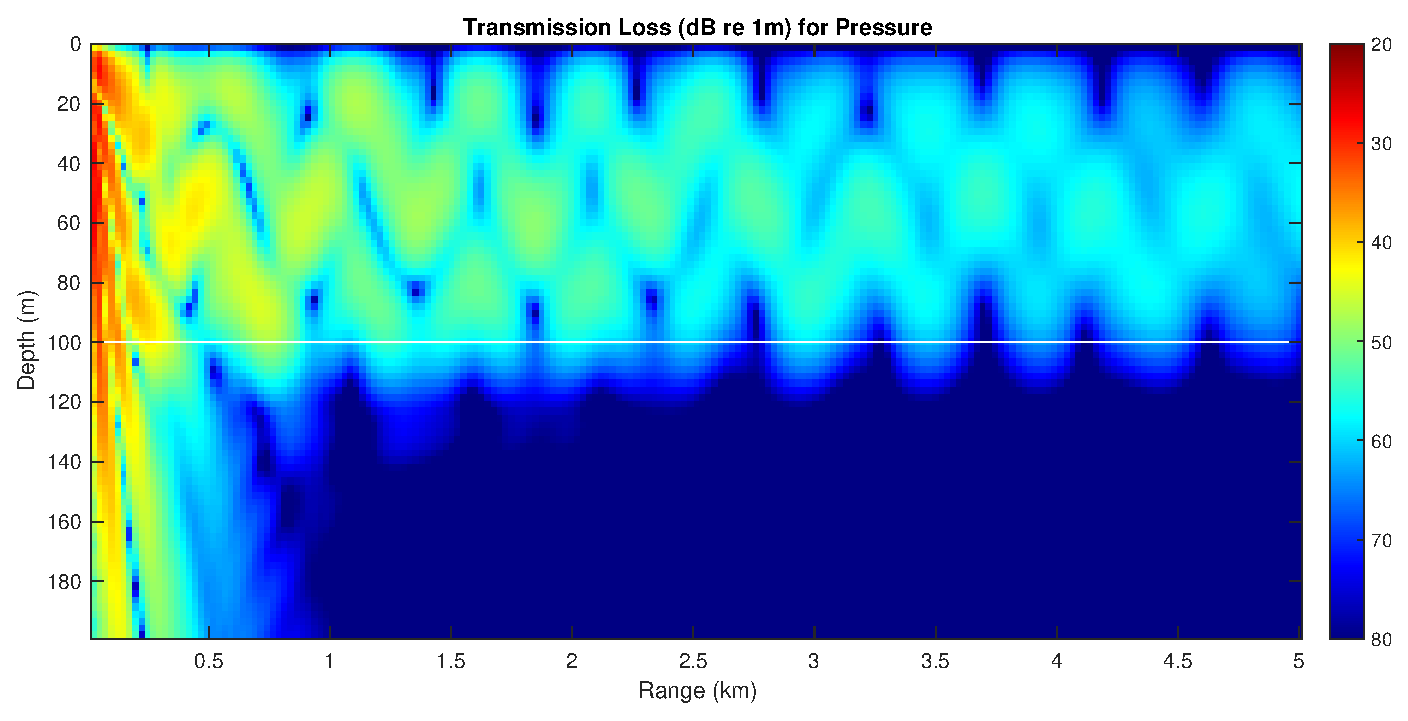
\includegraphics[width=\textwidth]{MonopoleP.eps}
\caption{\label{fig:MonopoleP}Monopole Source pressure transmission loss}
\end{center}
\end{figure}

\begin{figure}[!ht]
\begin{center}
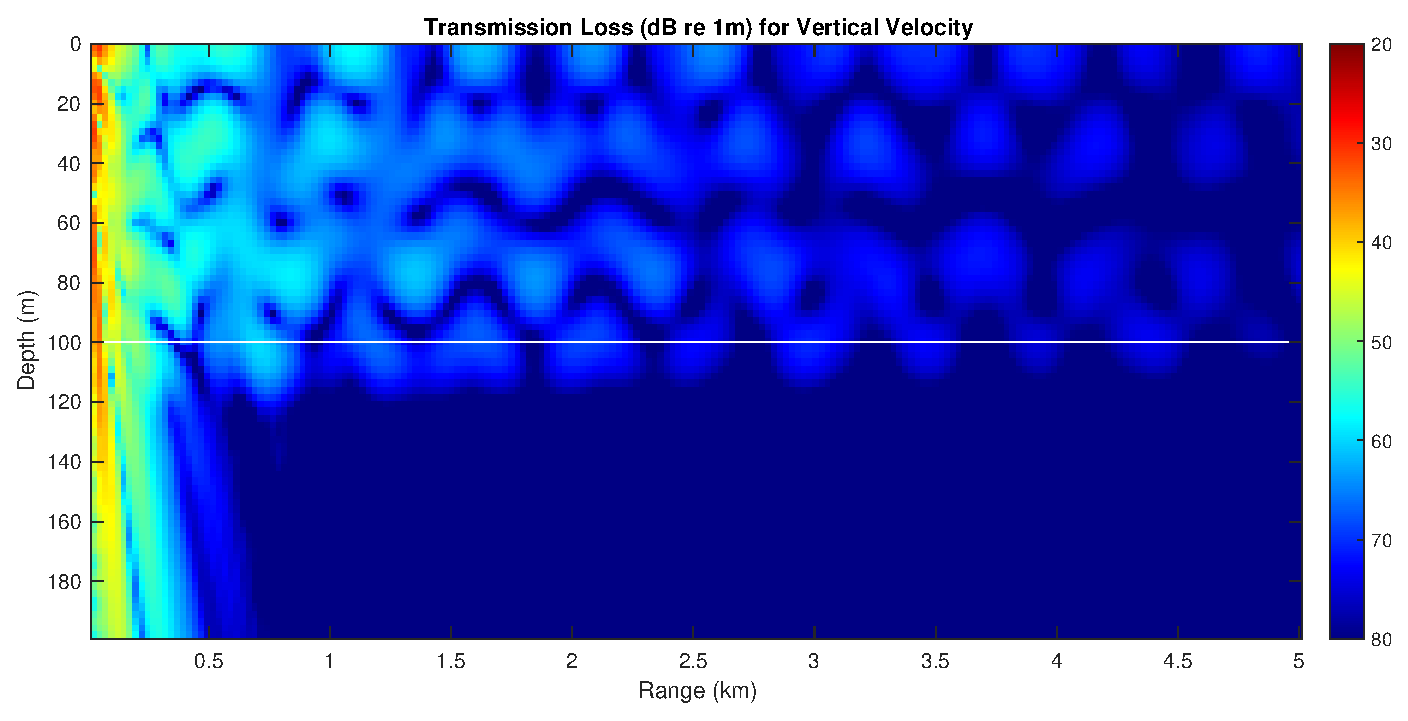
\includegraphics[width=\textwidth]{MonopoleVZ.eps}
\caption{\label{fig:MonopoleVZ}Monopole Source vertical velocity transmission loss}
\end{center}
\end{figure}

\clearpage
\subsubsection{Vertical Dipole Source}

This example demonstrates pressure and vertical velocity outputs for a vertical dipole source. It is identical to the Monopole example, except the source has been replaced with a vertical dipole.

\begin{figure}[!ht]
\begin{center}
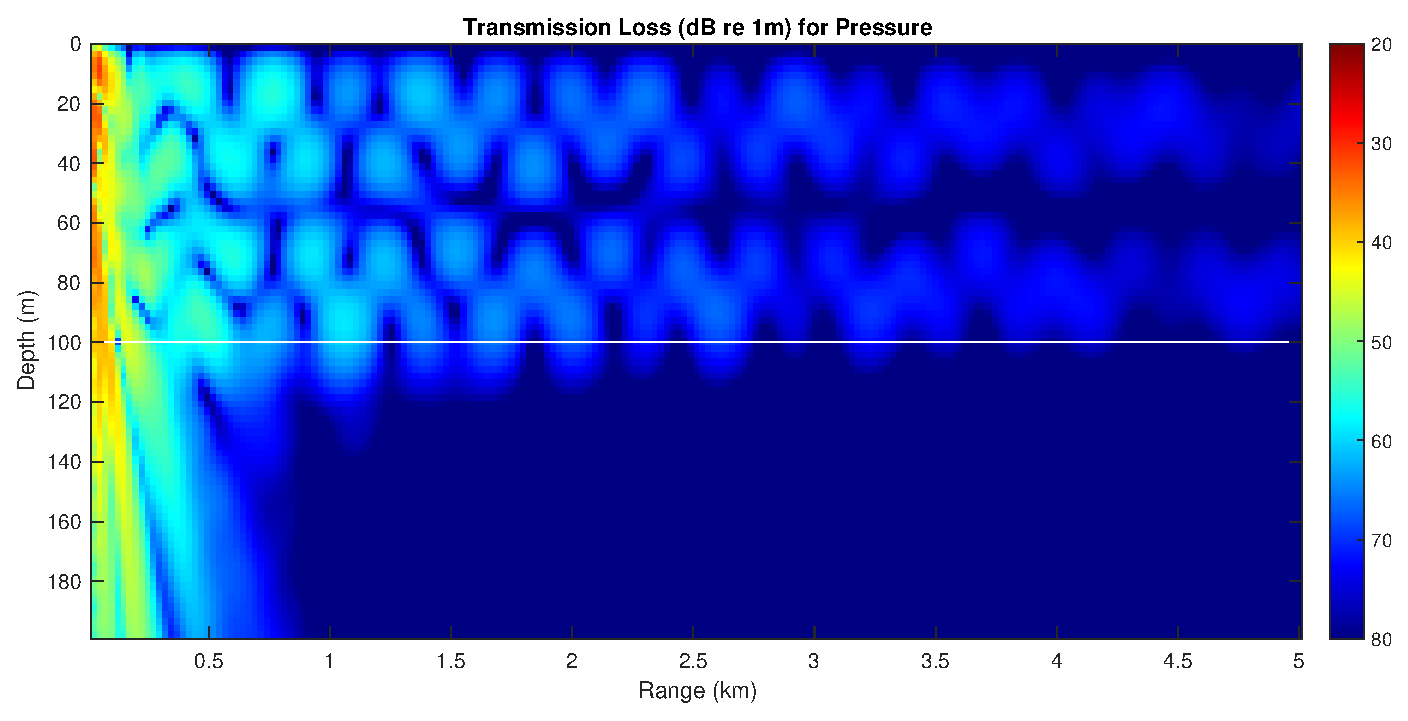
\includegraphics[width=\textwidth]{DipoleP.eps}
\caption{\label{fig:DipoleP}Vertical Dipole Source pressure transmission loss}
\end{center}
\end{figure}

\begin{figure}[!ht]
\begin{center}
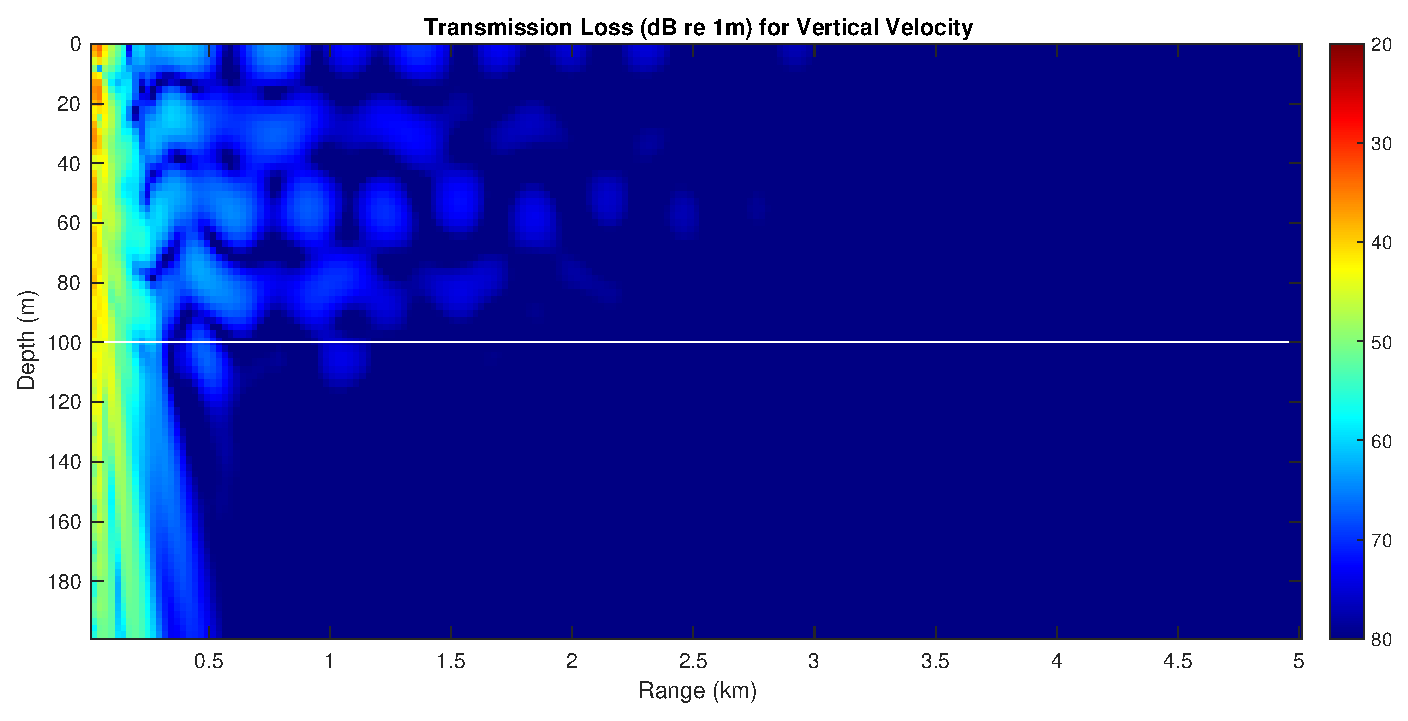
\includegraphics[width=\textwidth]{DipoleVZ.eps}
\caption{\label{fig:DipoleVZ}Vertical Dipole Source vertical velocity transmission loss}
\end{center}
\end{figure}

\clearpage
\subsubsection{Rough Surface}

This example demonstrates the effects of a rough ocean surface. It repeats the Flat environment example with a Pierson-Moskowitz surface wave spectrum for 20 m/s wind speed.

\begin{figure}[!ht]
\begin{center}
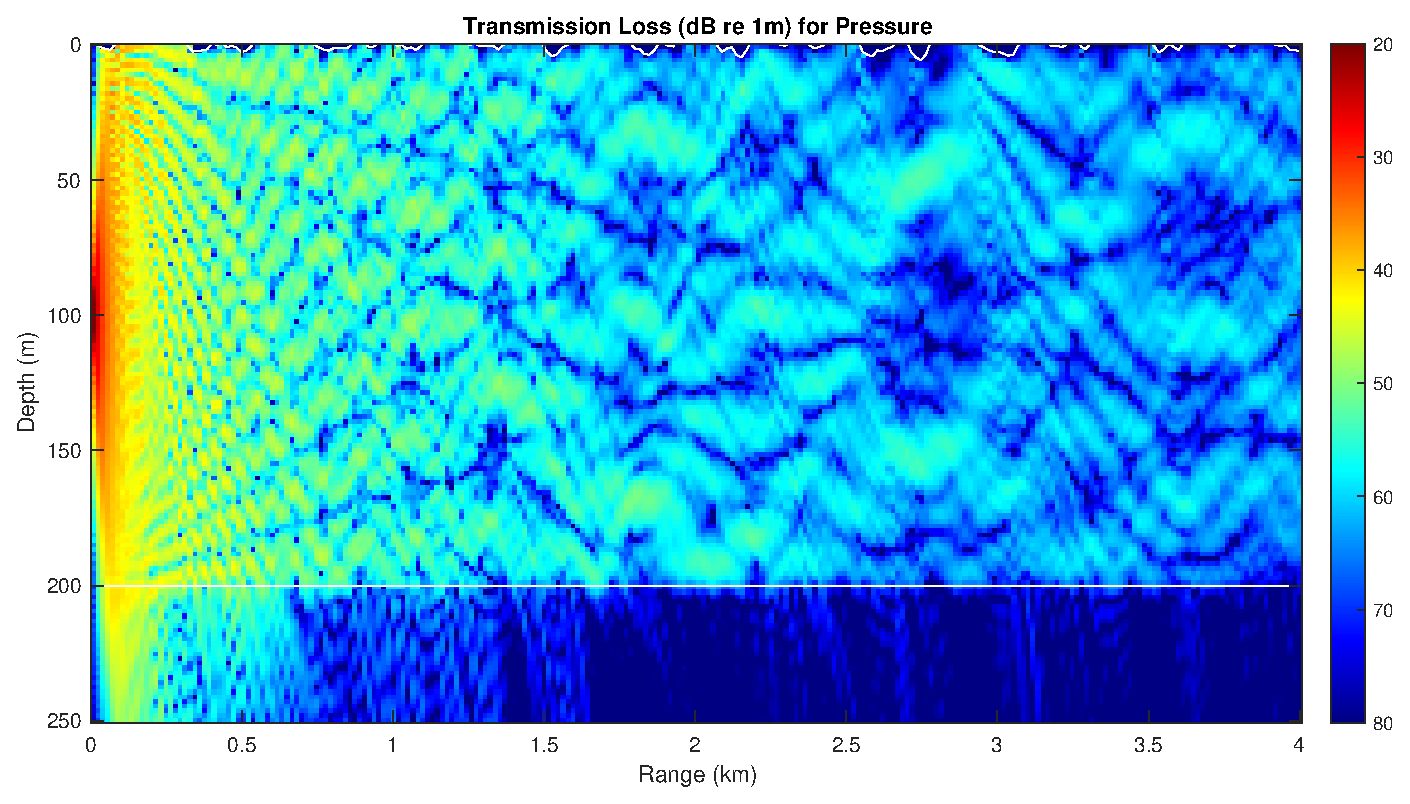
\includegraphics[width=\textwidth]{RoughSurfaceP.eps}
\caption{\label{fig:RoughSurfaceP}Flat environment with rough surface pressure transmission loss}
\end{center}
\end{figure}

\clearpage
\subsubsection{Travel Time}

The travel time example uses the Flat environment, but the source is now broadband. Its center frequency is 500 Hz, with 256 frequencies spanning a bandwidth of 255 Hz. The plot is for a range of 1 km.

\begin{figure}[!ht]
\begin{center}
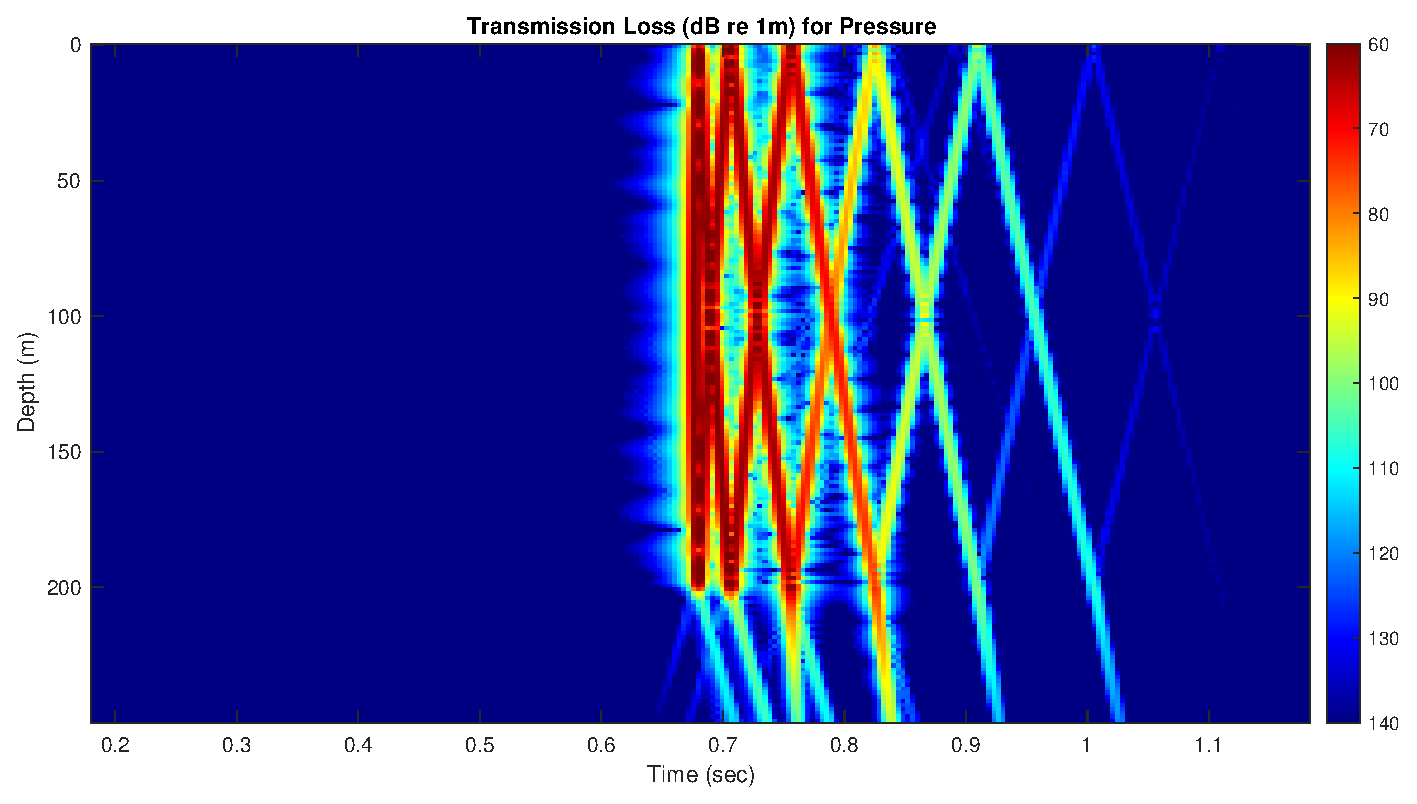
\includegraphics[width=\textwidth]{TravelTimeP.eps}
\caption{\label{fig:TravelTimeP}Flat environment pressure travel time}
\end{center}
\end{figure}
